\documentclass[tikz,border=5pt]{standalone}
\usepackage{amsmath,amssymb}
\begin{document}
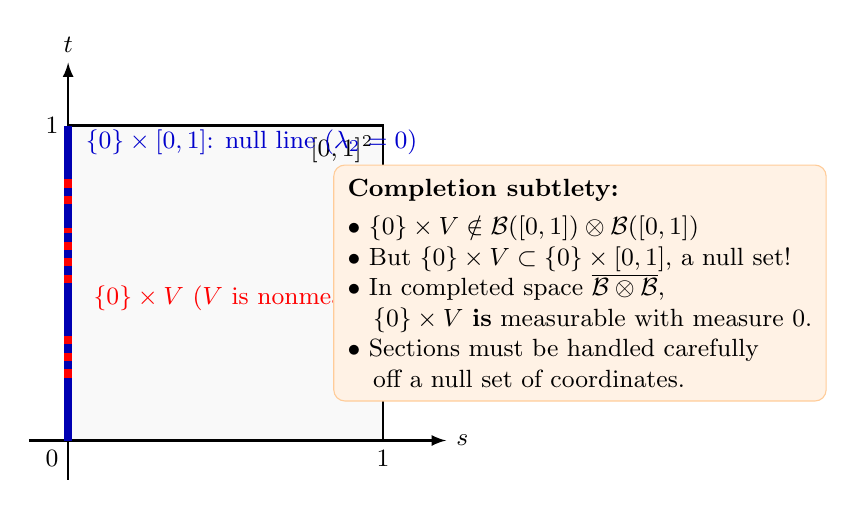
\begin{tikzpicture}[>=latex, font=\small]
  % Unit square
  \draw[thick, fill=gray!5] (0, 0) rectangle (4, 4);
  \node[anchor=north east] at (4, 4) {$[0,1]^2$};

  % Axes
  \draw[->, thick] (-0.5, 0) -- (4.8, 0) node[right] {$s$};
  \draw[->, thick] (0, -0.5) -- (0, 4.8) node[above] {$t$};

  \node[below left] at (0, 0) {$0$};
  \node[below] at (4, 0) {$1$};
  \node[left] at (0, 4) {$1$};

  % Vertical slice {0} x [0,1]
  \draw[line width=3pt, blue!70!black] (0, 0) -- (0, 4);
  \node[anchor=south west, blue!80!black] at (0.1, 3.5) {$\{0\} \times [0,1]$: null line ($\lambda_2 = 0$)};

  % Vitali subset {0} x V
  \draw[line width=3pt, red, dashed] (0, 0.8) -- (0, 1.4);
  \draw[line width=3pt, red, dashed] (0, 2.0) -- (0, 2.7);
  \draw[line width=3pt, red, dashed] (0, 3.0) -- (0, 3.4);
  \node[anchor=west, red] at (0.2, 1.8) {$\{0\} \times V$ ($V$ is nonmeasurable)};

  \node[align=left, fill=orange!10, draw=orange!40, rounded corners, inner sep=5pt] at (6.5, 2.0)
    {\textbf{Completion subtlety:}\\[3pt]
     $\bullet$ $\{0\} \times V \notin \mathcal{B}([0,1]) \otimes \mathcal{B}([0,1])$\\
     $\bullet$ But $\{0\} \times V \subset \{0\} \times [0,1]$, a null set!\\
     $\bullet$ In completed space $\overline{\mathcal{B} \otimes \mathcal{B}}$,\\
     \quad $\{0\} \times V$ \textbf{is} measurable with measure $0$.\\
     $\bullet$ Sections must be handled carefully\\
     \quad off a null set of coordinates.};
\end{tikzpicture}
\end{document}
